\chapter{Systementwurf}\label{chp:systementwurf}
%Auf der Basis des Pflichtenhefts werden aus softwaretechnischer Sicht die Anforderungen an das System spezifiziert. Hierzu gehört minimal eine Beschreibung auf höherem Niveau (Modulebene), eine auf mittlerem Niveau (Struktogramme, Pseudocode oder Spezifikation von Prozeduren (Funktionen) sowie die Beschreibung der für das System essentiellen Datenstrukturen (z.B. als Datenlexikon). Typische Beschreibungen sind die Modulhierarchie (oder Modulgraph), eine Spezifikation aller Module mit ihren Schnittstellen (inklusive Zweck, Ein-/Ausgabe), sowie eine Spezifikation aller in den Modulschnittstellen liegenden Prozeduren und Funktionen.
%Bestandteil des Entwurfs sollten nicht nur die jeweiligen Ergebnisse, sondern auch die Beschreibung des Entwicklungsweges (inklusive verworfener Lösungen) sein.

\section{Klasse Window}
\paragraph{}
Die Klasse \textit{Window} baut die Benutzeroberfläche auf und speichert die Eingabe des Benutzers in Variablen. Diese Werte werden dann an der Klasse \textit{Interpreter} weiter gegeben. In der Benutzeroberfläche werden die Eigenschaften für ein Testvorgang eingestellt.


\subsection{Design}
\begin{figure}[h]
  \begin{center}		%width=\linewidth
    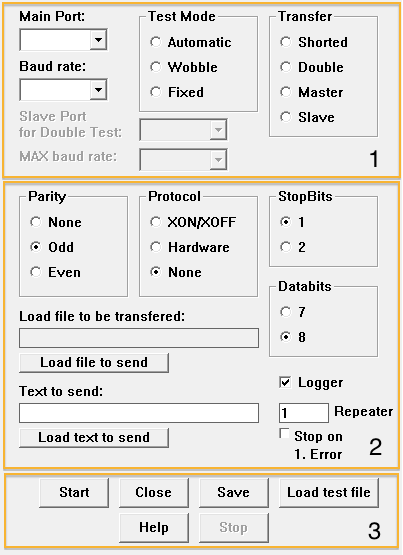
\includegraphics[scale=0.5]{gui.png}
  		  \caption{Design der Benutzeroberfläche}
  		  %\footnotesize{Quelle: www.pololu.com}
     \label{fig.3pi-m3pi-Module}
  \end{center}
\end{figure}


\paragraph{}
Die Benutzeroberfläche ist in drei Abteilungen geteilt. Die verschidene Abteilungen sind in Abbildung 5.1 zu erkennen. Genaueres zu alle Parametern wird in Kapitel ~\ref{chp:bedienungsanleitung} und  ~\ref{chp:fachlichesumfeld} erläutert. Die erste Reihe von Einstellungen hantieren die Testeinstellungen. Diese Einstellung sind:
\begin{itemize}
\item Main Port: welches COM Port soll getestet werden.
\item Baud rate: beschreibt mit welcher Baudrate der ausgewählte Port getestet werden soll.
\item Test Mode: definiert welcher Testvorgang der Benutzer haben will.
\item Transfer: legt fest, wie die Kommunikation dieses Ports stattfinden wird.
\end{itemize}

\paragraph{}
Die zwei ausgegraute Einstellungen ("`Slave Port for Double Test"' und "`MAX baud rate"') sind abhängig vor der Einstellungen in "`Test Mode"' und "`Transfer"'. 

\paragraph{}
Die zweite Abteilung von Einstellungen sind die Übertragungsparameter und drei weitere Testeinstellungen. Diese Parameter sind:
\begin{itemize}
\item Parity: Paritätsüberprüfung.
\item Protocol: Übertragungsprotokoll.
\item Stopbits: Anzahl der Stopbits.
\item Databits: Anzahl der Datenbits.
\item Logger: definiert ob eine Log-Datei erstellt werden soll.
\item Repeater: Anzahl der Testwiederholungen.
\item Stop on 1. Error: bestimmt ob bei der ersten Fehlererkennung angehalten werden soll.
\item Load file to be transfered: Übertragungsdatei.
\item Text to send: Übertragungstext.
\end{itemize}

\paragraph{}
Die letzte Reihe von Elemente in der Benutzeroberfläche sind die Knöpfe. Diese führen die jeweilige Vorgange aus.
\begin{itemize}
\item Start: startet ein Test.
\item Close: schließt das Test Tool.
\item Save: speichert in eine Testdatei die Einstellungen.
\item Load test file: ladet eine Datei die im Test übertragen wird.
\item Help: zeigt ein Fenster mit Erklärungen zum Test Tool.
\item Stop: stoppt der laufende Test.
\end{itemize}

\paragraph{}
Bei drücken des Start-, Save- oder "`Load test file"'knopfes werden die Testeinstellungen an die Klasse \textit{Interpreter} weitergegeben und dort werden diese verarbeitet.


\subsection{Aufbau}

\paragraph{}
Die Klasse hinter der Benutzeroberfläche besteht aus zwei Teilen. Das erste Teil bearbeitet die Eingabe des Benutzer und der Aufbau der Oberfläche, das zweite Teil die Weitererarbeitung der Daten.

\paragraph{}
Das erste Teil besteht aus die Methode \textit{HandleMessage}, diese Methode ist die Fensterprozedur. Als erstes werden die Elemente, mit der Ankunft der Nachricht \textit{WM\_CREATE},des Fensters aufgebaut. Danach wird auf die Nachricht \textit{WM\_COMMAND} gewartet und jeweils reagiert. Wird zum Beispiel das Start Knopf gedrückt, bekommt die \textit{HandleMessage} die \textit{WM\_COMMAND} Nachricht mit dem Parameter \textit{ID\_BT\_START}. Das ist die Identifikationsnummer im Programm für das Start Knopf.

\paragraph{}
Wenn der Start Knopf gedrückt worden ist, fängt das zweite Teil der Klasse an. Das zweite Teil besteht aus die Weiterverarbeitung der Eingaben. Im Fall vom Start Knopf, wird als erstes einen neuen Thread aufgerufen. So kann die Benutzeroberfläche immer noch Nachrichten verarbeiten, während im Hintergrund, das Programm die Datenverarbeitung beginnt. Der gleiche Vorgang geschieht, wenn der \textit{Load test file} gedrückt wird.

\paragraph{}
Im Fall vom Start Knopf, ruft das Thread die Methode \textit{sendTestSettings} auf, die die Eingaben weiter gibt. Dies geschieht in dem ein Objekt der Klasse \textit{Interpreter} erzeugt wird und dessen Eigenschaften werden gesetzt.



\lstset{language=C++,
				backgroundcolor=\color{light-gray},
				%frame=single,
				tabsize=2,
				numbers=left,
				numbersep=5pt,
				%numberstyle=\color{light-gray},
				basicstyle=\ttfamily\color{black}\small,
				keywordstyle=\color{HKS51}\bfseries,
				commentstyle=\color{HKS13}\slshape,,
				identifierstyle=\color{black}}
\begin{lstlisting}	

LRESULT Window::HandleMessage(UINT uMsg, WPARAM wParam, LPARAM lParam)
{
    switch (uMsg)
    {

    case WM_CREATE:
        {
            //Create al GUI Elements
            
            //example: Start button
            _hwnd_Start = CreateWindowA("button", "Start",
				WS_CHILD | WS_VISIBLE,
				POS_X+20, POS_Y2 + 290, 70, 30, m_hwnd, (HMENU)ID_BT_START,
				NULL, NULL);
        }
        break;
        
    case WM_COMMAND:
        {
            //React to GUI Elements actions
            
            //example: Start button
            case ID_BT_START:

				//hide the elements while testing
				viewAllElements(FALSE);

				//start a new thread
				_t1 = thread(&Window::sendTestSettings, this);
				
				//detach the thread so it can test and main thread waits for it to finish
				//or waits for the user to press stop
				_t1.detach();
        }
        break;
        
    case WM_DESTROY:
        PostQuitMessage(0);
        break;

	//call the default window procedure for the other messages
    default:
        return DefWindowProc(m_hwnd, uMsg, wParam, lParam);
    }
    return TRUE;
}

\end{lstlisting}





\section{Klasse Interpreter}
\paragraph{}

\subsection{}





\section{Struktur TestStruct}
\paragraph{}

\subsection{}






\section{Klasse Com}
\paragraph{}

\subsection{}


\section{Klasse PortCommunications}
\paragraph{}

\subsection{}



\section{Klasse TestManager}
\paragraph{}

\subsection{}


\section{Klasse FixedTest}
\paragraph{}

\subsection{}


\section{Klasse IniFileHandler}
\paragraph{}

\subsection{}


\section{Klasse Logger}
\paragraph{}

\subsection{}


\section{Klasse Tools}
\paragraph{}

\subsection{}


\section{Klasse TransferFileHandler}
\paragraph{}

\subsection{}